
\section{Testing}

In this section, we will test the performance of our strategies by comparing their profit rate and portfolio values. We will also go over the testing that we perform on the trading simulation software to ensure that it operates as expected.

\subsection{Trading Simulation Software}

The trading simulation software has a few unit tests that ensure that certain operations are working correctly. The virtual portfolio is tested with a unit test that performs operations on a portfolio instance and checks that the output of each operation is as expected. That is, it tests all of the transaction methods with valid and invalid inputs, making sure that the correct output is returned each time. We also perform unit tests on \texttt{TradingContext} to ensure that it delivers events to the strategies in order. This test is implemented by defining several mock trading event emitters that emit a mock trading event class that only contains a timestamp. The test also defines a trading strategy that accumulates all of the events that it receives and an assertion is performed at the end to make sure that all of the events occur in the expected order. We perform unit testing on the \texttt{MarketEventsEmitter} to make sure that the market open/close events are only sent for days when the market is open. It also ensures that a market open event is always followed by a market close event on the same day. This unit test is performed with a hardcoded time range (so that we can manually figure out a list of events that should be emitted and easily compare this with the result).

As a precaution, we also perform extensive logging during the execution of a simulation, so that it is possible to detect any issues by looking back at logs. This has allowed us to detect issues that are harder to write tests for, such as incorrect author weight calculation in the opinion aggregation implementation.

\subsection{Trading Strategy Performance}

Trading strategies are tested by running a simulation with historical data and observing their performance. This performance can be analyzed to determine which strategies are performing the best, and which ones perform the worst.

We tested 7 different strategies, including the baseline strategy and the buy-and-hold S\&P 500 strategy. The ``Moving Average'' and ``Moving Average with Sentiment'' strategies detailed in the refinement report were also tested. Additionally, three variations of the ``Selection by Sentiment'' strategy were tested. The first is ``SelectionBySentiment(OneStock)'', which is the ``Selection by Sentiment'' strategy with $n=1$. ``SelectionBySentiment(AllStocks)'' is the ``Selection by Sentiment'' strategy with $n=11$. ``SelectionBySentiment'' is the ``Selection by Sentiment'' strategy with $n=3$. A graph of each strategy's portfolio values over time for the year of 2014 is shown in figure~\ref{allStrategiesGraph}.

\begin{figure}[h]
  \label{allStrategiesGraph}
  \begin{center}
    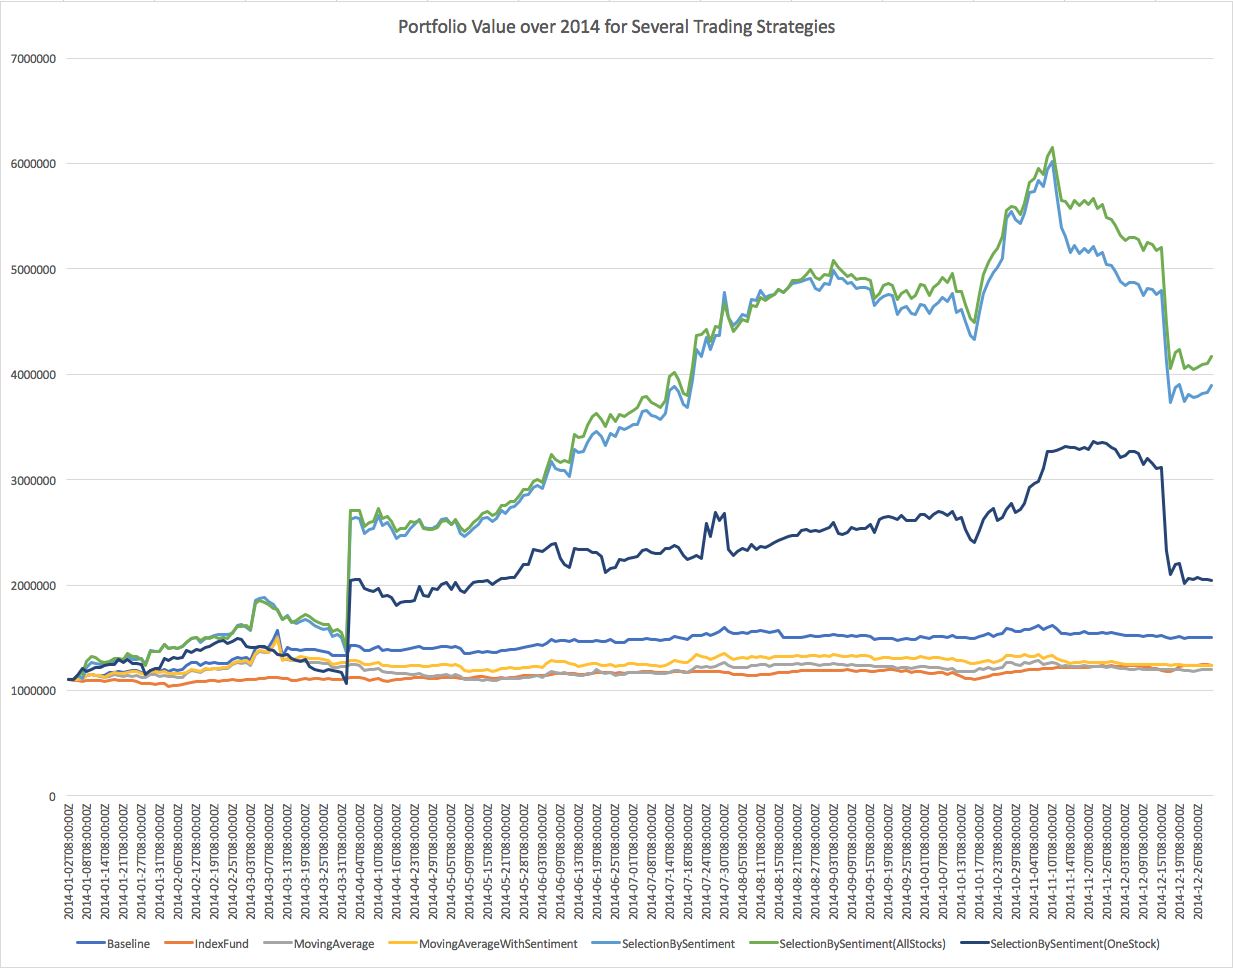
\includegraphics[max width=\textwidth]{allStrategiesGraph}
  \end{center}
  \caption{A graph of the portfolio values for the year of 2014 for several trading strategies.}
\end{figure}

The Moving Average strategy only shows some marginal improvement over the S\&P 500 index. By considering the sentiment with the moving average, we see some additional improvement over that, but unfortunately, the Moving Average with Sentiment strategy yields lower returns than our baseline implementation.

The Selection by Sentiment strategy yields the greatest returns of any strategy that we have tested by far. Interestingly (and maybe intuitively), greater values of  n  yield a higher return, even though this disagrees with the assertion made by the related work \cite{tradingSentimentPaper}.

We start each strategy off with a total of \$1.1 million. The ``SelectionBySentiment(AllStocks)'' strategy’s maximum portfolio value over the year was \$6.15 million (on Nov 10th), which is an incredible 459\% profit. This strategy closed the year (on Dec 31st) with \$4.17 million (a 279\% profit) after dropping quite a bit in a short time frame, but this number is still significantly higher than any other strategy.

There is a large jump in the graph for all Selection by Sentiment strategies from April 1st to April 2nd. After some analysis, we discovered that this due to an investment in the MNKD stock (which was \$4.02 on April 1st and closed at \$6.99 on April 2nd). This occurred because MNKD received a recommendation for FDA approval from an assembled Adcom committee after two previous denials from the FDA. Looking at the posts from our StockTwits data on March 31st, we received an influx of speculative posts about FDA approval (like ``@the\_\_twit \texttt{\$MNKD} , I fully expect to get at least partial approval, but more importantly-soon Europe will also approve. Insulin lab there+2'' and ``\texttt{\$MNKD} in the end with approval I expect that it will shove it into the 7.87 range.-then fade-as people come to grips with the work ahead..'').

There was also a large fall-off towards the end of the year on December 16th. This was due to the purchase of \texttt{\$VRNG} on December 12th in anticipation of the Federal Circuit’s ruling on Vringo’s request for en banc. This request was denied by the Federal Circuit on December 15th, sending the stock into a free-fall. After looking at the StockTwits posts from December 11th, some seemed to be hopeful that the en banc would be approved, while others seemed pessimistic. Here are some examples of these posts: ``\texttt{\$VRNG} Thus far charts looking nicely. We may take a nice rise.'', ``\texttt{\$VRNG} I’m here. Good morning VRNGites! Hope Mr Buies is ready to deal with corupt system and we go to \$10!!!!'', ``\texttt{\$VRNG} Chief Judge Prost has stood up for the little guy in the past...  \url{http://stks.co/e1MT6}'', and ``\texttt{\$VRNG} Trying to get licensing fees from ZTE is like stopping piracy. It’s not going to happen, and def not for a significant amt of money.'' These posts give some insight into what’s happening, but there doesn’t seem to be a clear consensus. This indicates that experimentation with the cutoffs for bullish and bearish aggregated opinions could improve performance.

\subsection{Additional Refinements}

In the future, we'd like to further refine our system by adding more comprehensive support for corporate actions like stock splits and dividends without having to hardcode them in our simulation. Our goal is to perform more testing, specifically with data from the year of 2015. This will help us determine whether our strategy is scalable or if it is market-dependent. We would also like to add support for volume information and more complex and realistic stock ordering mechanisms in our simulation software. Our current simulation makes the assumption that the volume of stock that we would like to buy is available for purchase and that the volume of stock that we would like to sell is always sold. This is not always true in the real world, and it requires a more complicated simulation that takes the trading volumes into account to model this phenomenon. A more realistic simulation might support realistic ordering mechanisms like market orders and limit orders and implement slippage models like Quantopian does \cite{quantopianSlippage}. On top of this, we'd like to experiment with machine learning based strategies that perform price prediction based on sentiment and past price trends. More long-term refinements might include full support for live testing with real-time data, integration with real trading platforms like Robinhood \cite{robinhood} and the Bloomberg Terminal \cite{terminal}. 

%%% Local Variables:
%%% mode: latex
%%% TeX-master: "../report"
%%% End:
